\section{Pré-processamento dos dados}

Para que os algoritmos tenham uma maior eficácia, é necessário que os dados fornecidos pelo desafio sejam processados. Esse processamento é responsável por excluir dados que prejudiquem o aprendizado, preencher os faltantes (quando possível), criação de novas colunas, compilando e/ou combinando as características já existentes e, se necessário, manipulação dos dados para simplificação de categorias, com o objetivo de tornar o conjunto de dados mais enxuto.

\subsection{Tratamento de Outliers}

Um dos passos importantes para o tratamento de dados, é a identificação e remoção de pontos muito fora do padrão, para que o algortimo não se atrapalhe com pontos que não fazem parte do conjunto de dados normalmente, que tem pouca ocorrência.

No caso desse desafio, o próprio autor do dataset indica que existem outliers no conjunto de dados de treino.

Podemos observar os outliers no gráfico abaixo.

\lstset {
  backgroundcolor=\color{white}, 
   basicstyle=\tiny,       
  breakatwhitespace=false,
  breaklines=true,
  captionpos=b,
   commentstyle=\color{red},
   frame=single,
   keepspaces=true,
   language=Python,
   numbers=left,
   numbersep=5pt,
   numberstyle=\tiny\color{gray},
   showspaces=false,
   showstringspaces=false,
   showtabs=false,
   stepnumber=1,
   stringstyle=\color{mauve},
   tabsize=1,
}
\begin{lstlisting}
import matplotlib.pyplot as plt 
import pandas as pd

df_train=pd.read_csv('./input/train.csv')

fig, ax = plt.subplots()
ax.scatter(x = df_train['GrLivArea'], y = df_train['SalePrice'])
plt.ylabel('SalePrice', fontsize=13)
plt.xlabel('GrLivArea', fontsize=13)
plt.show()

\end{lstlisting}

\begin{figure}[H]
	\centering
	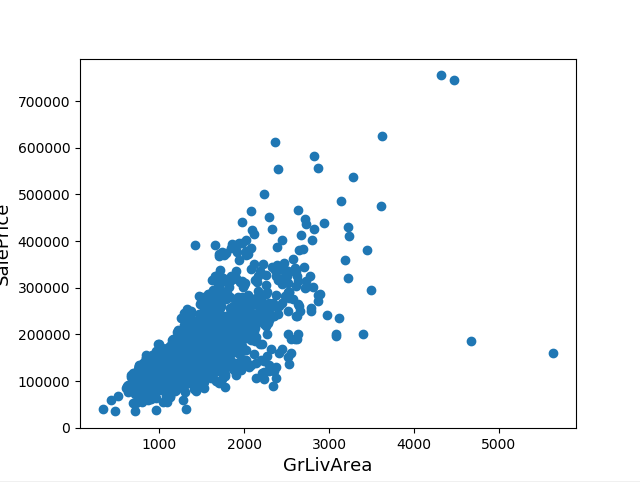
\includegraphics[keepaspectratio,width=1\textwidth]{img/outlier.png}
\end{figure}

O autor recomenda remover os dois pontos que tem uma grande área, e que foram vendidos por um preço muito baixo. Que são os dois pontos com $ GrLivArea > 4.000 $ \& $ SalePrice < 300.000 $.

\lstset {
  backgroundcolor=\color{white}, 
   basicstyle=\tiny,       
  breakatwhitespace=false,
  breaklines=true,
  captionpos=b,
   commentstyle=\color{red},
   frame=single,
   keepspaces=true,
   language=Python,
   numbers=left,
   numbersep=5pt,
   numberstyle=\tiny\color{gray},
   showspaces=false,
   showstringspaces=false,
   showtabs=false,
   stepnumber=1,
   stringstyle=\color{mauve},
   tabsize=1,
}
\begin{lstlisting}
df_train = df_train.drop(df_train[(df_train['GrLivArea']>4000) & (df_train['SalePrice']<300000)].index)

fig, ax = plt.subplots()
ax.scatter(x = df_train['GrLivArea'], y = df_train['SalePrice'])
plt.ylabel('SalePrice', fontsize=13)
plt.xlabel('GrLivArea', fontsize=13)
plt.show()

\end{lstlisting}

\begin{figure}[H]
	\centering
	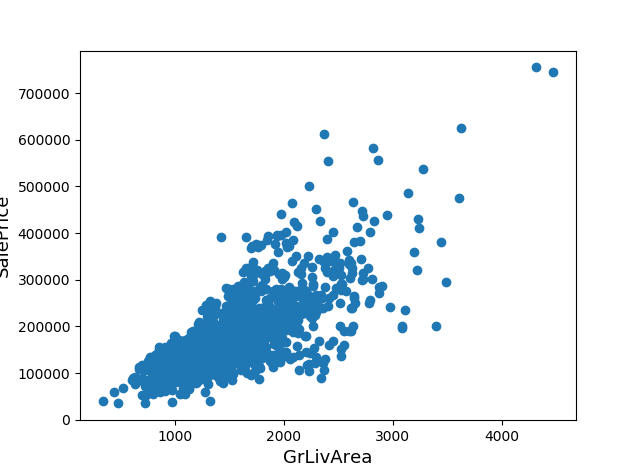
\includegraphics[keepaspectratio,width=1\textwidth]{img/outlier-retirados.png}
\end{figure}

\subsection{Variável Alvo}

Como dito anteriormente, a variável a ser calculada é o preço do imóvel. Sendo assim, é necessário avaliar a relação do SalePrice com as outras variáveis do conjunto de dados, e também a sua normalização.


\lstset {
  backgroundcolor=\color{white}, 
   basicstyle=\tiny,       
  breakatwhitespace=false,
  breaklines=true,
  captionpos=b,
   commentstyle=\color{red},
   frame=single,
   keepspaces=true,
   language=Python,
   numbers=left,
   numbersep=5pt,
   numberstyle=\tiny\color{gray},
   showspaces=false,
   showstringspaces=false,
   showtabs=false,
   stepnumber=1,
   stringstyle=\color{mauve},
   tabsize=1,
}
\begin{lstlisting}
sns.distplot(df_train['SalePrice'] , fit=norm);

# Get the fitted parameters used by the function
(mu, sigma) = norm.fit(df_train['SalePrice'])
print( '\n mu = {:.2f} and sigma = {:.2f}\n'.format(mu, sigma))

#Now plot the distribution
plt.legend(['Normal dist. ($\mu=$ {:.2f} and $\sigma=$ {:.2f} )'.format(mu, sigma)],
            loc='best')
plt.ylabel('Frequency')
plt.title('SalePrice distribution')

#Get also the QQ-plot
fig = plt.figure()
res = stats.probplot(df_train['SalePrice'], plot=plt)
plt.show()

\end{lstlisting}

\begin{figure}[H]
	\centering
	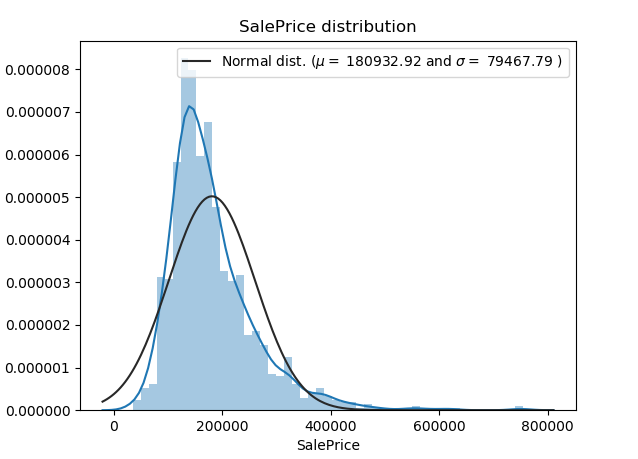
\includegraphics[keepaspectratio,width=1\textwidth]{img/saleprice-normalizado.png}
\end{figure}

\begin{figure}[H]
	\centering
	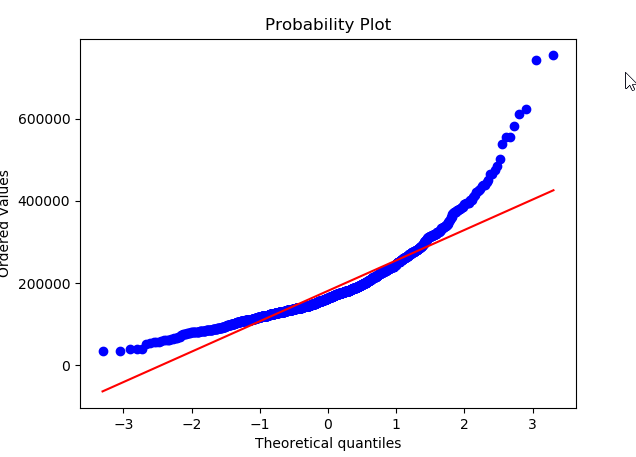
\includegraphics[keepaspectratio,width=1\textwidth]{img/saleprice-prob.png}
\end{figure}

Como podemos perceber, a variável é \textit{skewed} positivamente. Com isso, para que os regressores lineares funcionem de uma melhor forma, é importante que a variável seja normalizada. Mas é importante lembrar que, para submeter a resposta para avaliação, é nessário reverter o log para o preço normal.


\lstset {
  backgroundcolor=\color{white}, 
   basicstyle=\tiny,       
  breakatwhitespace=false,
  breaklines=true,
  captionpos=b,
   commentstyle=\color{red},
   frame=single,
   keepspaces=true,
   language=Python,
   numbers=left,
   numbersep=5pt,
   numberstyle=\tiny\color{gray},
   showspaces=false,
   showstringspaces=false,
   showtabs=false,
   stepnumber=1,
   stringstyle=\color{mauve},
   tabsize=1,
}
\begin{lstlisting}
df_train["SalePrice"] = np.log1p(df_train["SalePrice"])

\end{lstlisting}

\begin{figure}[H]
	\centering
	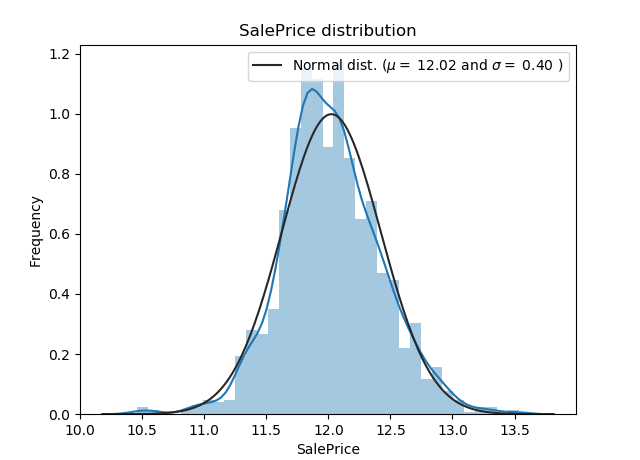
\includegraphics[keepaspectratio,width=1\textwidth]{img/saleprice-norm.png}
\end{figure}

\begin{figure}[H]
	\centering
	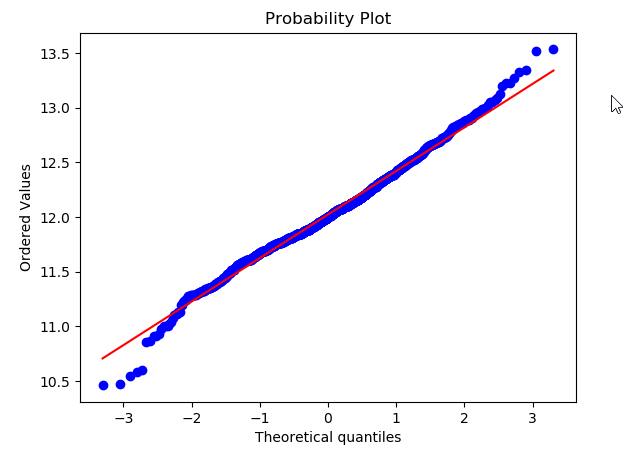
\includegraphics[keepaspectratio,width=1\textwidth]{img/saleprice-prob-norm.png}
\end{figure}

\clearpage